% ---------------------------------------------------------------
% 6. Implementação
% ---------------------------------------------------------------
\chapter{Implementação}\label{cap:implementacao}

\section{Arquitetura}\label{sec:arquitetura}

A arquitetura utilizada separa o mundo simulado, a perceção e o conhecimento (Figura 16). O WorldState contém tudo o que existe no cenário, mas o motor de inferência só conhece o que os sensores detetaram. Toda a política de decisão está nas regras; o código Java simula, encaminha eventos e aplica decisões, e a interface apenas apresenta e envia comandos. A Tabela 8 apresenta os principais componentes, com base em dois princípios:

\begin{itemize}
  \item \textbf{A cada} 100 ms é executado um ciclo; todos os pedidos REST passam por métodos sincronizados do SimulationEngine
  \item \textbf{Comandos por REST, estado por \ing{WebSocket}.} Cada comando tem a sua resposta; o
        estado completo é enviado para o \ing{browser} a cada ciclo.
\end{itemize}

\begin{figure}[htbp]
\centering
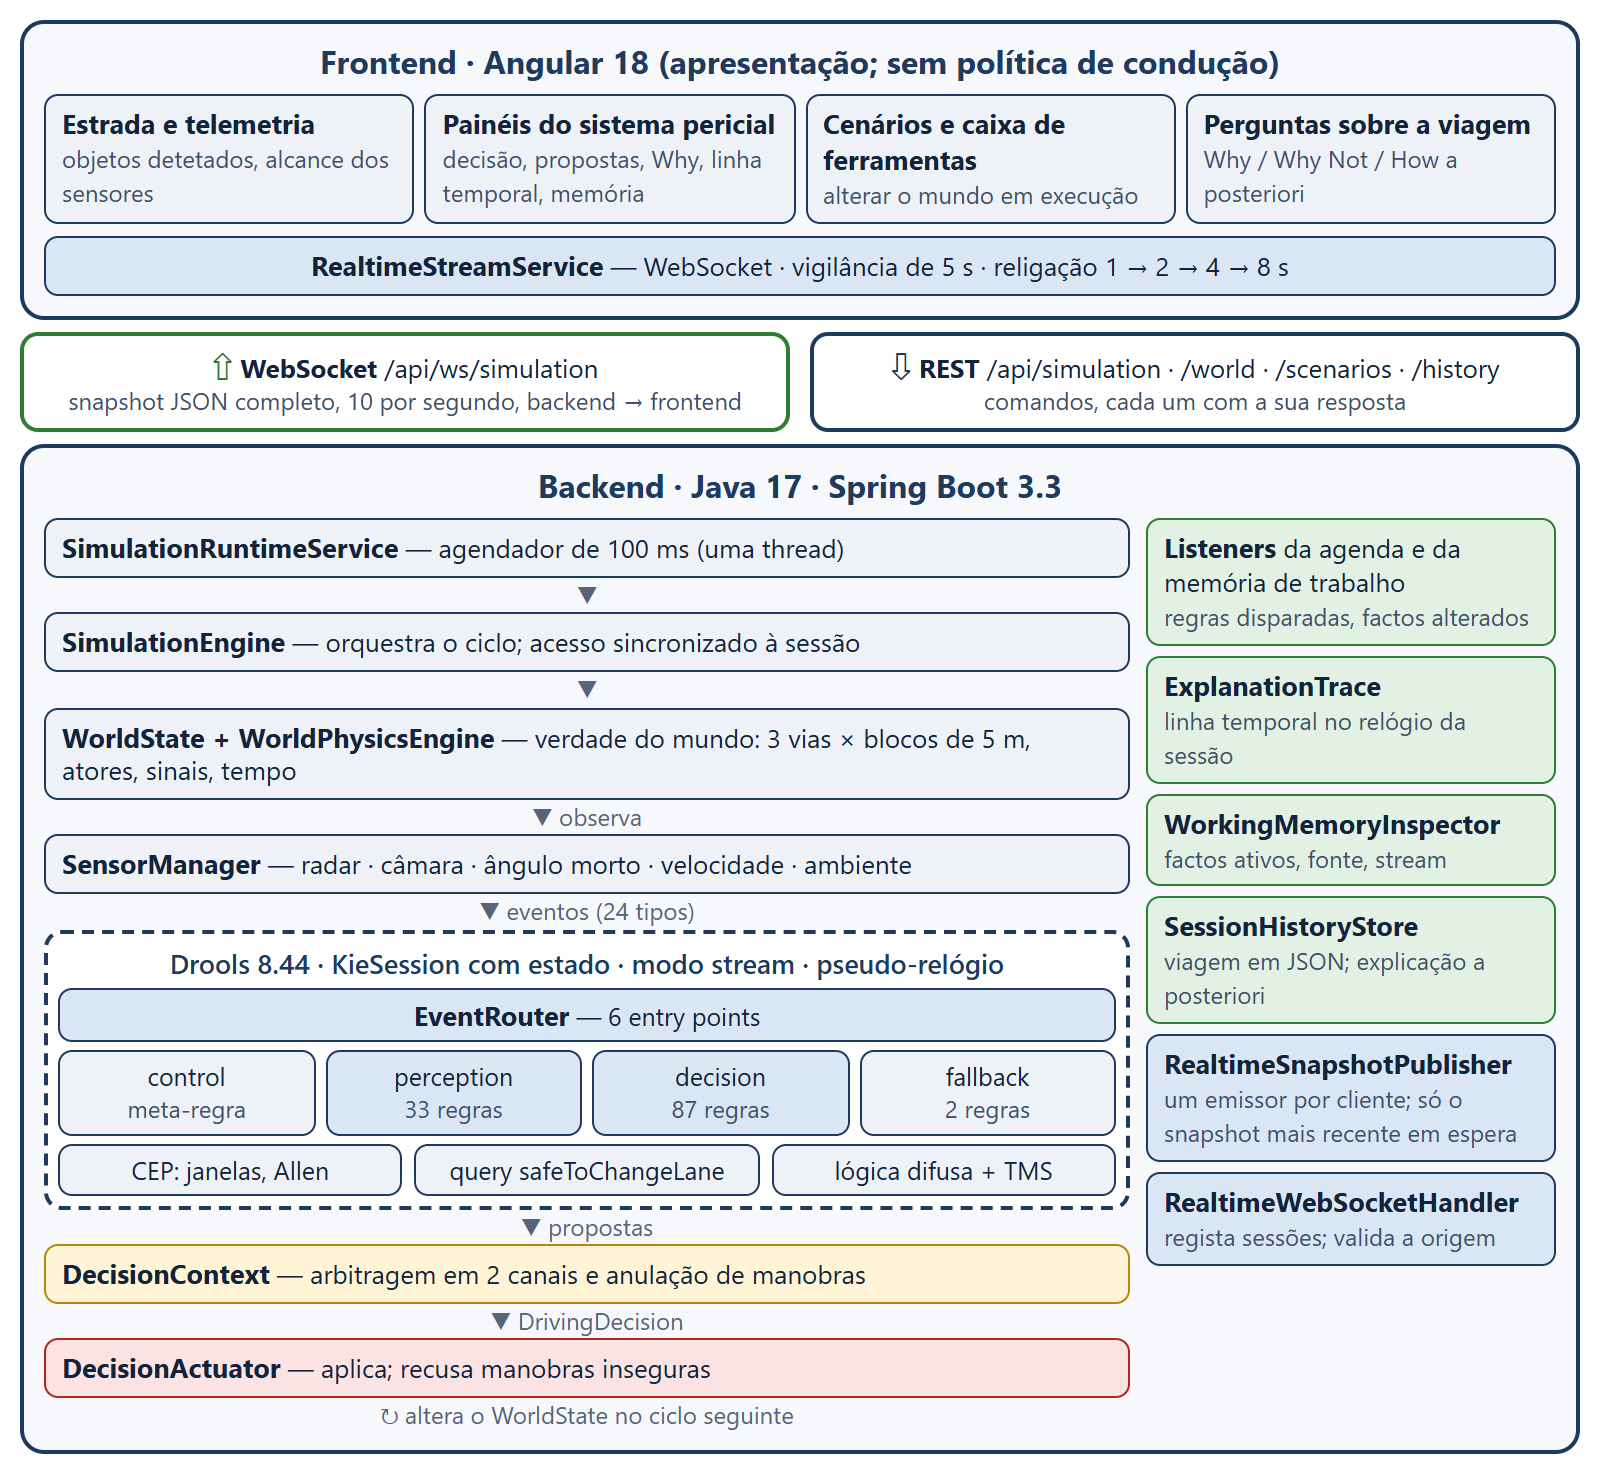
\includegraphics[width=0.92\textwidth,height=0.62\textheight,keepaspectratio]{figuras/arquitetura.png}
\caption{Arquitetura do sistema e fluxo de informação}
\label{fig:arquitetura}
\end{figure}

\begin{table}[htbp]
\centering
\small
\caption{Componentes principais}\label{tab:componentes}
\rowcolors{2}{white}{corFundo}
\begin{tabular}{@{}L{0.33\textwidth}L{0.61\textwidth}@{}}
\linhacab \cab{Componente} & \cab{Responsabilidade} \\
\cod{SimulationRuntimeService} & Agendador de 100 ms; constrói o \ing{snapshot} de cada ciclo e entrega-o ao publicador \\
\cod{SimulationEngine} & Responsável pelo ciclo; arranque, pausa, paragem, cenários e alterações ao mundo \\
\cod{WorldState} · \cod{WorldPhysicsEngine} & Mundo simulado (estrada em matriz, veículos, peões, sinais, tempo) e a sua evolução física \\
\cod{SensorManager} & Os cinco sensores, cada um com cadência e alcance próprios \\
\cod{EventRouter} · \cod{KnowledgeSession} & Encaminham os eventos para os \ing{entry points} e gerem a \cod{KieSession} \\
\cod{DecisionContext} & Recolhe as propostas do ciclo e arbitra-as por canal, registando o destino de cada uma \\
\cod{DecisionActuator} & Aplica a decisão (aceleração, pisca, mudança de via) e recusa manobras inseguras \\
\cod{ExplanationTrace} · \ing{listeners} & Linha temporal das regras e dos factos; inspetor da memória de trabalho \\
\cod{SessionHistoryStore} & Grava cada viagem em JSON e responde a \ing{Why}, \ing{Why Not} e \ing{How} a posteriori \\
\cod{RealtimeSnapshotPublisher} & Envia o \ing{snapshot} a cada \ing{browser} ligado, sem nunca bloquear a simulação \\
\end{tabular}
\end{table}

\begin{table}[htbp]
\centering
\small
\caption{Tecnologias utilizadas}\label{tab:tecnologias}
\rowcolors{2}{white}{corFundo}
\begin{tabular}{@{}L{0.17\textwidth}L{0.29\textwidth}L{0.48\textwidth}@{}}
\linhacab \cab{Componente} & \cab{Tecnologia} & \cab{Utilização} \\
\ing{Backend} & Java 17, Spring Boot 3.3.4 & Simulação, sensores, motor de inferência e API REST/\ing{WebSocket} \\
Motor de regras & \ing{Drools} / KIE 8.44 & Sessão com estado, regras DRL, CEP, encadeamento progressivo e consultas \\
\ing{Frontend} & Angular 18, RxJS & Visualização da simulação e dos painéis do sistema pericial \\
Comunicação & \ing{WebSocket} e REST & Estado em tempo real (\ing{WebSocket}) e comandos (REST) \\
Testes & JUnit 5, Jasmine/Karma, Playwright & Regras, arbitragem, ciclo de simulação, integração e testes de ponta a ponta \\
\end{tabular}
\end{table}

\FloatBarrier
\section{O ciclo de 100 ms}\label{sec:ciclo}

A Figura 17, a título de exemplo, mostra, por ordem, o que acontece em cada ciclo.

\begin{figure}[htbp]
\centering
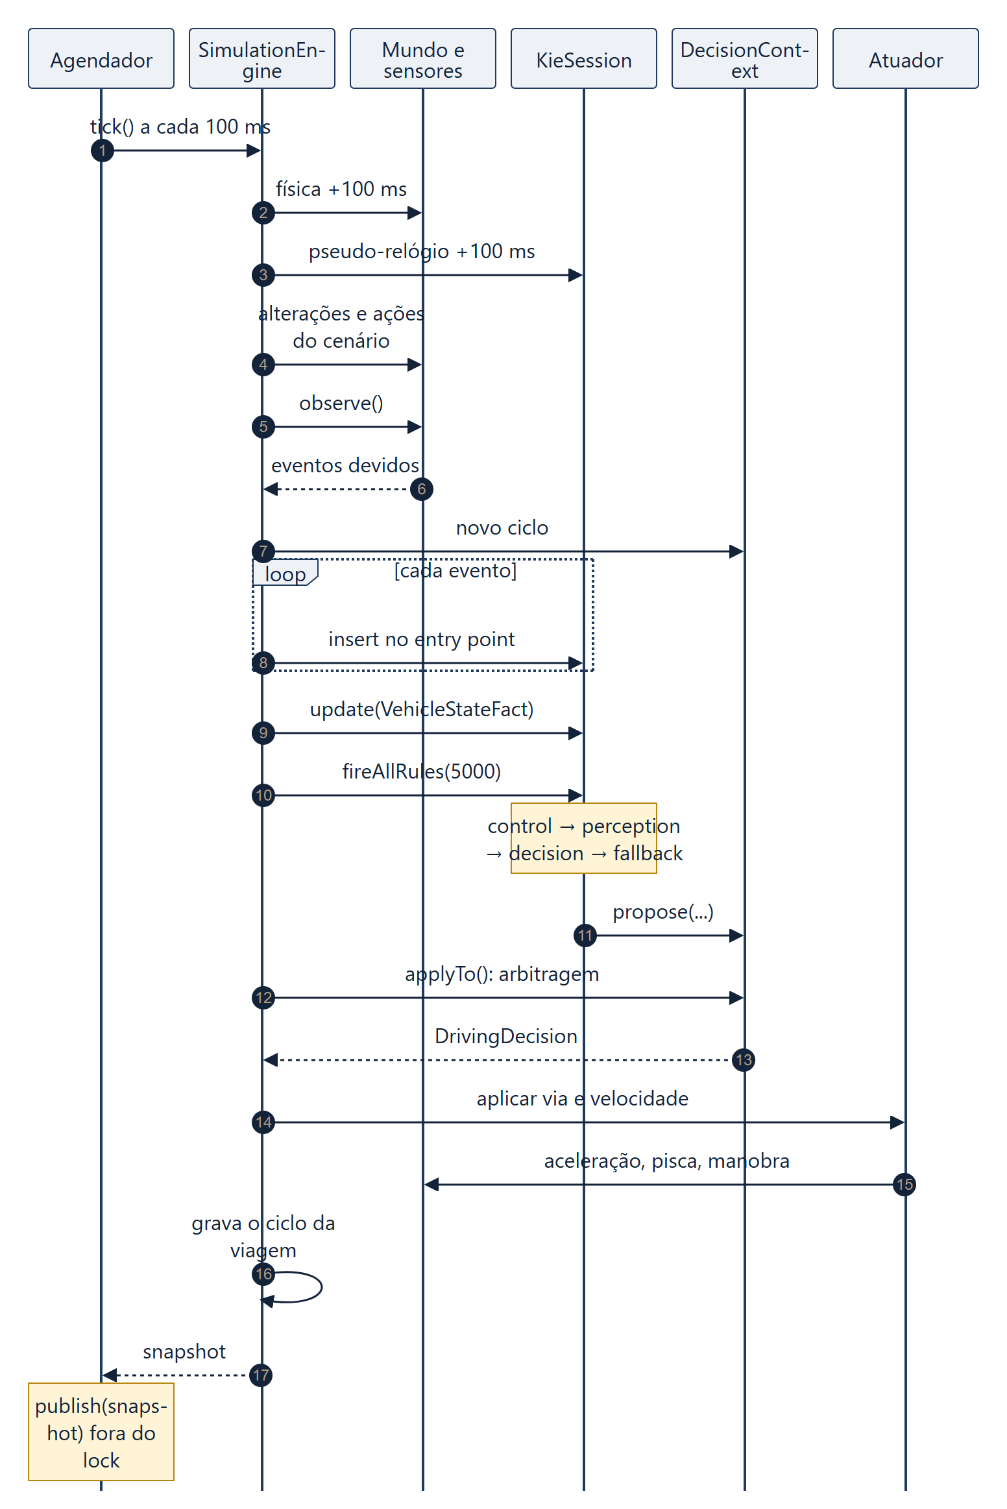
\includegraphics[width=\textwidth,height=0.80\textheight,keepaspectratio]{figuras/ciclo_simulacao.png}
\caption{Sequência de um ciclo de simulação}
\label{fig:ciclo-simulacao}
\end{figure}

\FloatBarrier
\section{O motor de inferência}\label{sec:motor}

\textbf{Entry points.} Os eventos entram por seis fluxos com nome (Tabela 10), o que separa semanticamente a origem da informação e permite às regras temporais ler só o fluxo de que precisam.

\begin{table}[htbp]
\centering
\small
\caption{\ing{Entry points} e eventos encaminhados}\label{tab:entrypoints}
\rowcolors{2}{white}{corFundo}
\begin{tabular}{@{}L{0.30\textwidth}L{0.64\textwidth}@{}}
\linhacab \cab{\ing{Entry point}} & \cab{Eventos} \\
\cod{VEHICLE\_STREAM} & Velocidade do veículo \\
\cod{PERCEPTION\_STREAM} & Distância, velocidade relativa e TTC; peões; ocupação das vias laterais; veículos nas vias vizinhas \\
\cod{ROAD\_STREAM} & Sinais de limite e de STOP, passadeiras, buracos, obstáculos, barreiras \\
\cod{TRAFFIC\_STREAM} & Estado dos semáforos \\
\cod{ENVIRONMENT\_STREAM} & Chuva, visibilidade e aderência \\
\cod{COMMAND\_STREAM} & Pedidos de aceleração e de mudança de via \\
\end{tabular}
\end{table}

Metaconhecimento de controlo. As regras encontram-se organizadas em grupos (Tabela 11), cuja execução é controlada por uma meta-regra.

\begin{table}[htbp]
\centering
\small
\caption{Grupos de agenda}\label{tab:grupos}
\rowcolors{2}{white}{corFundo}
\begin{tabular}{@{}L{0.16\textwidth}C{0.09\textwidth}L{0.67\textwidth}@{}}
\linhacab \cab{Grupo} & \cab{Regras} & \cab{Função} \\
\cod{control} & 1 & Meta-regra «\ing{Control: perceive, then decide, then fall back}» (saliência 10000) \\
\cod{perception} & 33 & Eventos $\rightarrow$ factos de estado; expiração das perceções; lados seguros para mudar de via \\
\cod{decision} & 87 & Regras que propõem ações e mantêm estados intermédios (lógica difusa, arranque, ultrapassagem) \\
\cod{fallback} & 2 & Manter a velocidade se nada foi proposto; arrancar quando nada retém o veículo \\
\end{tabular}
\end{table}

\textbf{Raciocínio temporal (CEP).} Os 24 tipos de evento são declarados com @role(event), @timestamp e @expires (3 a 30 s), o que mantém a memória limitada.

\textbf{Encadeamento regressivo.} «É seguro mudar de via para este lado?» é um objetivo, definido por uma consulta que se prova a partir de quatro subobjetivos: maneuverIdle, noContinuousLine, sideClear e roomToFollow.


\textbf{Lógica difusa.} A visibilidade e a aderência são vagas, por isso são fuzzificadas em quatro termos (fraca, reduzida, razoável, boa) e combinadas por cinco regras difusas (E = mínimo, OU = máximo) como, por exemplo, com chuva, visibilidade 0,7 e aderência 0,65, o teto obtido é de cerca de 51 km/h. As pertenças e as conclusões difusas são inseridas com insertLogical: quando a leitura meteorológica muda, perdem a justificação e são retiradas pelo próprio motor.

\FloatBarrier
\section{Comunicação em tempo real: \ing{WebSocket}}\label{sec:websocket}

A interface tem de mostrar, dez vezes por segundo, o veículo, as deteções, a decisão dos dois canais, todas as propostas com o seu destino, a linha temporal e a memória de trabalho. Para isso, o backend mantém com cada browser uma ligação WebSocket em /api/ws/simulation e, a cada ciclo, envia por ela um snapshot JSON completo do sistema. A ligação é aberta uma vez e fica aberta: cada atualização é apenas uma frame de texto e chega à interface no próprio ciclo em que a decisão é tomada. O canal é usado num só sentido, do backend para o frontend, e sem protocolos adicionais (sem STOMP). Os comandos (iniciar, parar, carregar cenários, inserir elementos) continuam em REST (Tabela 12), porque cada um precisa da sua própria resposta e do seu código de erro; depois de cada comando, o backend envia logo um snapshot, para que o efeito apareça sem esperar pelo ciclo seguinte.

\begin{table}[htbp]
\centering
\small
\caption{Separação entre comandos (REST) e estado (\ing{WebSocket})}\label{tab:rest}
\rowcolors{2}{white}{corFundo}
\begin{tabular}{@{}L{0.52\textwidth}L{0.42\textwidth}@{}}
\linhacab \cab{Pedido} & \cab{Função} \\
\cod{POST /api/simulation/\{start | pause | resume | stop | reset\}} & Ciclo de vida da simulação \\
\cod{POST /api/scenarios/\{id\}/load} & Carregar um cenário \\
\cod{POST · PUT · DELETE /api/world/elements}, \cod{/api/world/actors} & Inserir, alterar ou remover elementos e atores durante a simulação \\
\cod{PUT /api/world/map/cells} & Pintar uma célula da matriz da estrada \\
\cod{POST /api/environment} & Mudar a meteorologia \\
\cod{GET /api/history/sessions} · \cod{POST \ldots/\{id\}/why} & Viagens gravadas e perguntas \ing{Why} / \ing{Why Not} / \ing{How} \\
\cod{ws://\ldots/api/ws/simulation} & Estado completo a cada ciclo e após cada comando \\
\end{tabular}
\end{table}

\textbf{Formato da mensagem.} Cada frame tem a forma \{"event":"snapshot","payload":\{\ldots\}\} e é serializada pelo mesmo ObjectMapper da API REST, pelo que é exatamente o mesmo JSON de GET /api/simulation/state. A Tabela 13 resume o conteúdo.

\begin{table}[htbp]
\centering
\small
\caption{Conteúdo de um \ing{snapshot}}\label{tab:snapshot}
\rowcolors{2}{white}{corFundo}
\begin{tabular}{@{}L{0.32\textwidth}L{0.62\textwidth}@{}}
\linhacab \cab{Campo} & \cab{Conteúdo} \\
\cod{egoVehicle} · \cod{environment} & Velocidade, posição, via, aceleração, estado da manobra, pisca; chuva, visibilidade e aderência \\
\cod{currentDecision} & Decisão de velocidade e de via, regra, razão, evidência, risco e prioridade; todas as propostas com o seu destino; resposta ao «porque não mudar de via» para cada lado \\
\cod{sensors} · \cod{detectedObjectIds} & Telemetria de cada sensor e os objetos realmente detetados pela câmara e pelo radar \\
\cod{worldObjects} · \cod{roadMap} & Elementos do mundo relativos ao veículo e a matriz da estrada \\
\cod{workingMemory} · \cod{recentTimeline} & Factos ativos (tipo, valor, fonte, \ing{stream}) e as últimas 160 entradas da linha temporal \\
\cod{status} · \cod{simulationTimeMillis} & Estado da simulação e tempo simulado \\
\end{tabular}
\end{table}

A Figura 18 mostra a ligação completa: o handshake, a validação da origem, o snapshot imediato, o envio periódico e a interação com os comandos REST. Como o CORS não se aplica a WebSockets, a origem é verificada no handshake: só a interface do projeto (http://localhost:4200) pode abrir o canal; outra origem recebe 403.

\begin{figure}[htbp]
\centering
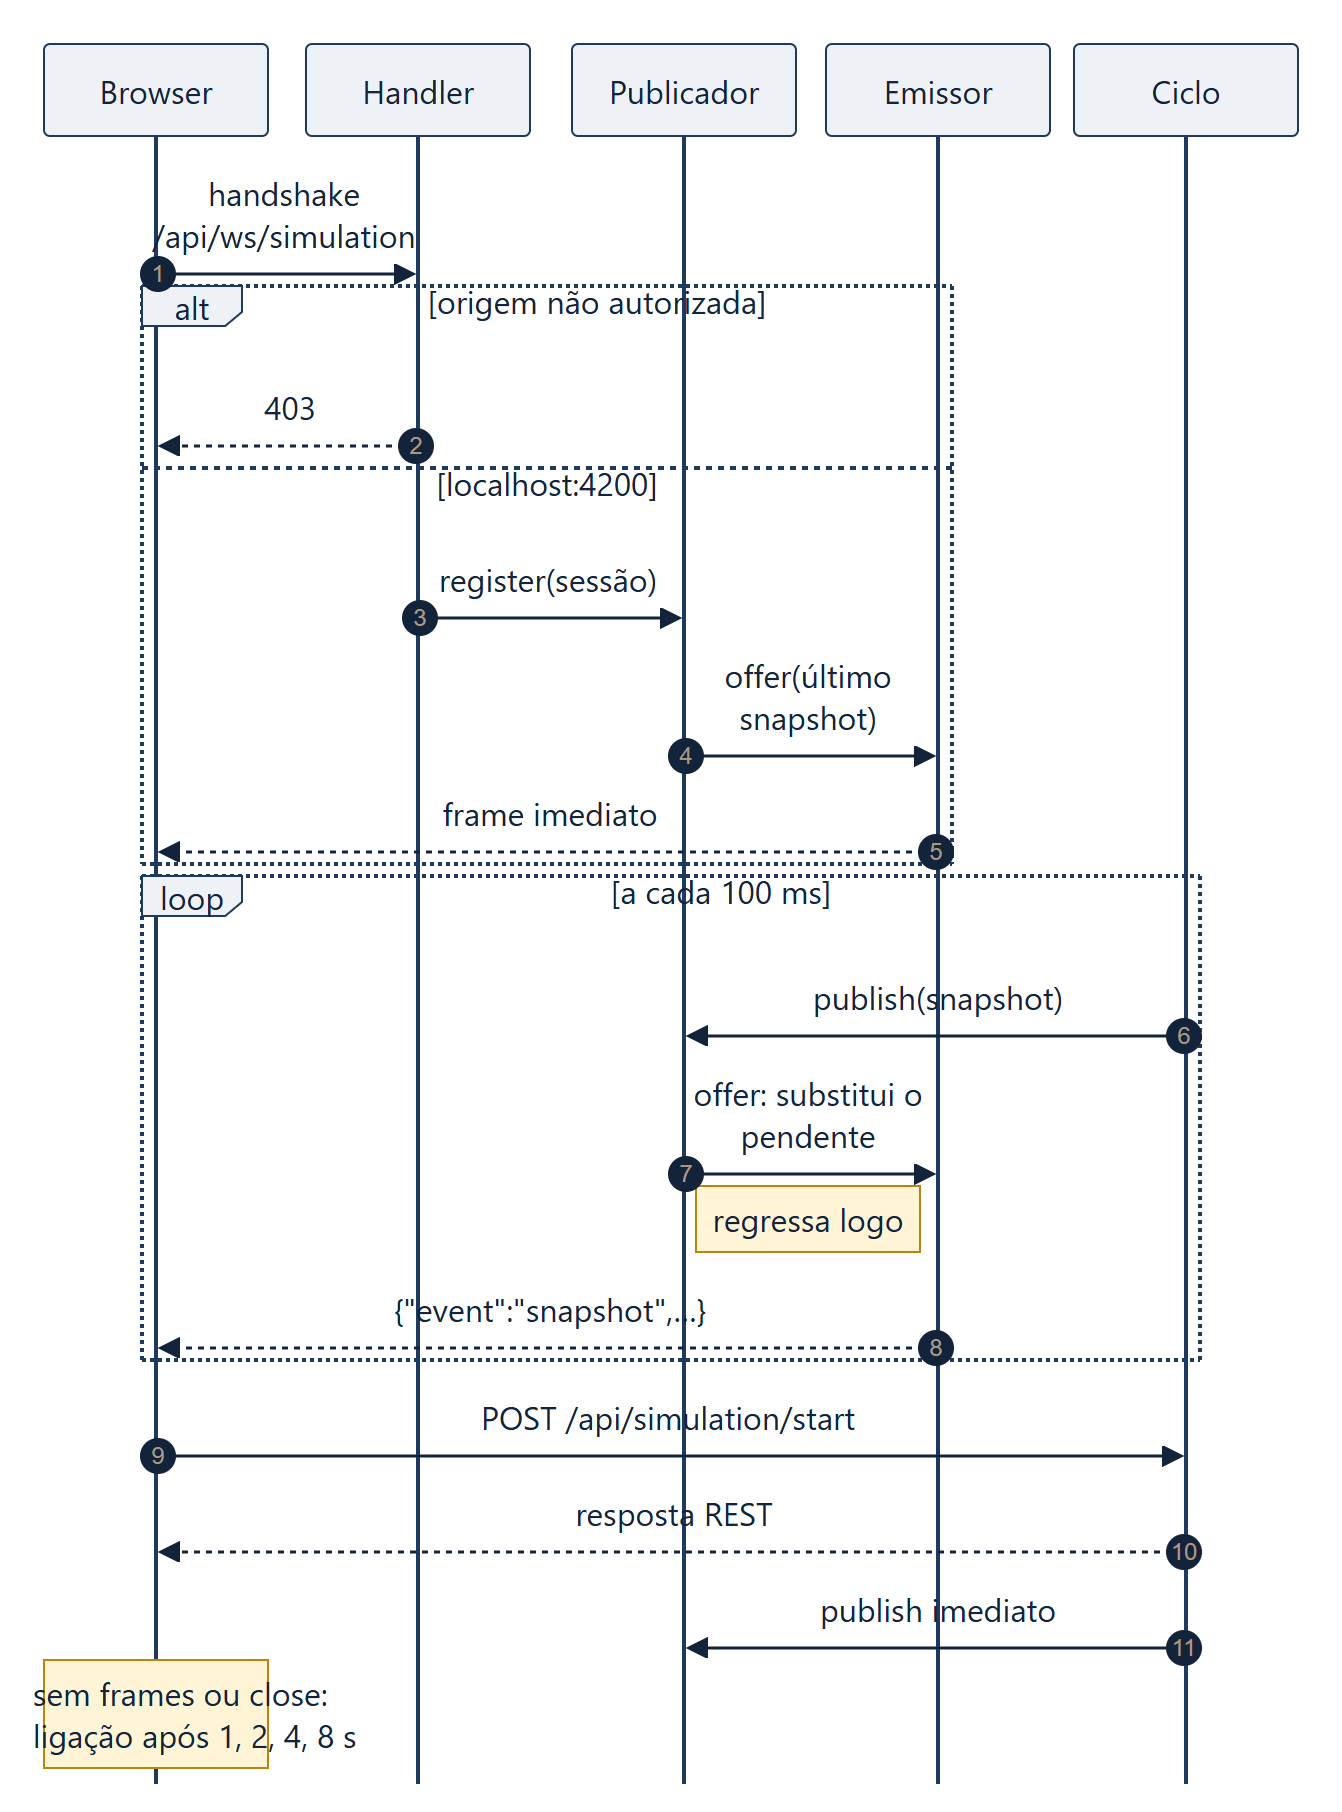
\includegraphics[width=\textwidth,height=0.78\textheight,keepaspectratio]{figuras/websocket_sequencia.png}
\caption{Sequência da ligação \ing{WebSocket} e da sua interação com os comandos REST}
\label{fig:ws-sequencia}
\end{figure}

A implementação resolve três problemas de um canal de tempo real:

\begin{itemize}
  \item \textbf{Um cliente lento não atrasa a simulação.} A publicação nunca espera pelo envio: cada navegador tem o seu emissor, com no máximo uma escrita em curso e apenas o snapshot mais recente em espera. Um separador em segundo plano perde frames intermédios, mas como cada snapshot é um estado completo não perde informação.
  \item \textbf{Entrada imediata.} Quem liga, ou volta a ligar, recebe logo o último snapshot, sem esperar pelo ciclo seguinte.
  \item \textbf{Recuperação automática.} O frontend considera a ligação morta se não receber frames durante 5 s e volta a ligar com esperas crescentes (1 s, 2 s, 4 s, até 8 s). A ligação valida a origem do pedido, para que só a interface do projeto a possa abrir.
\end{itemize}

Os três problemas são resolvidos em dois lados: no servidor, que nunca pode ficar à espera de um
\ing{browser}, e no cliente, que tem de perceber sozinho quando a ligação morreu.

\textbf{Servidor: um emissor por cliente.} Uma escrita bloqueante num socket de um browser lento (por exemplo, um separador em segundo plano) pararia o fio da simulação. Por isso, o RealtimeSnapshotPublisher dá a cada sessão o seu próprio emissor (Figura 19):

\begin{itemize}
  \item \cod{publish()} guarda o \ing{snapshot} e entrega-o a cada emissor; regressa de imediato e
        é chamado fora do \ing{lock} da simulação, pelo que os pedidos REST também nunca esperam
        pela rede;
  \item cada emissor tem uma só posição de espera (AtomicReference) e no máximo uma escrita em curso (AtomicBoolean): um snapshot novo substitui o que ainda não foi enviado. Um cliente lento perde frames intermédias, mas como cada frame é um estado completo nunca fica com informação errada;
  \item as escritas correm em \ing{threads} próprias (\cod{ws-sender}), o que também garante que
        uma \cod{WebSocketSession}, que não é segura entre \ing{threads}, recebe uma escrita de
        cada vez;
  \item o registo de um cliente novo e a publicação partilham um lock, pelo que nenhum cliente perde nem recebe fora de ordem um snapshot concorrente;
  \item se uma escrita falhar ou expirar, o cliente é removido e a sessão fechada; um erro de
        serialização descarta apenas essa \ing{frame}.
\end{itemize}

\begin{figure}[htbp]
\centering
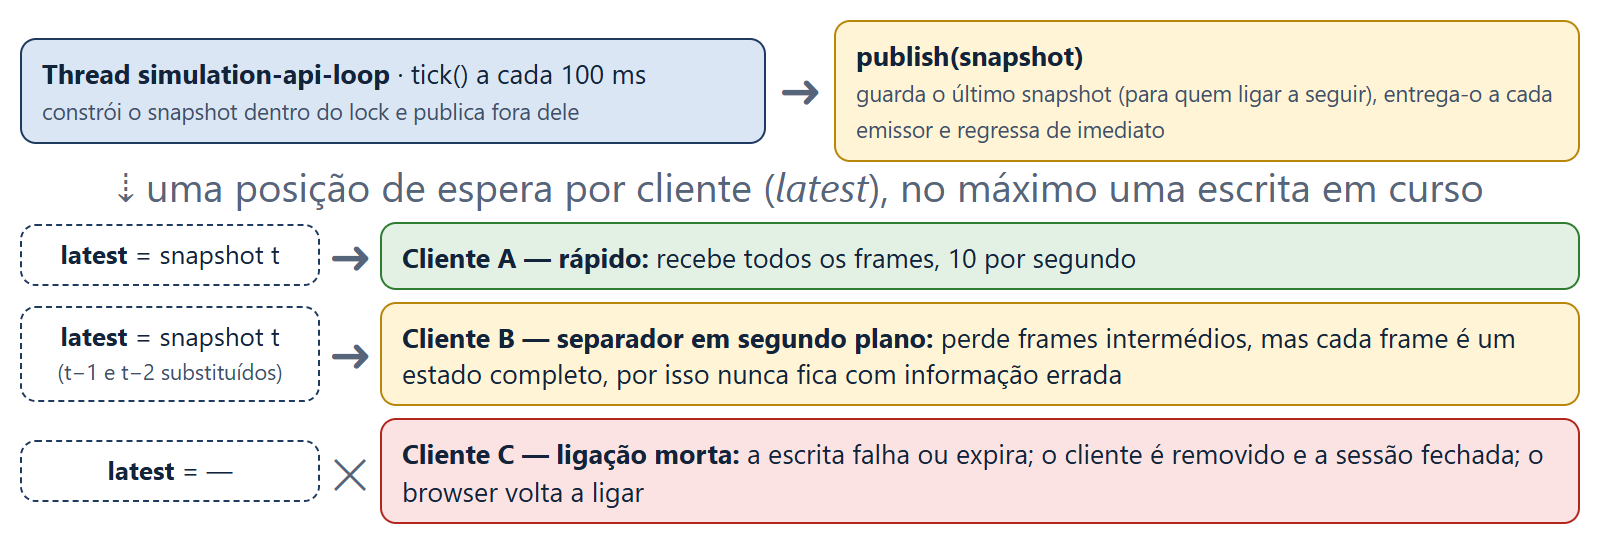
\includegraphics[width=\textwidth]{figuras/websocket_publicador.png}
\caption{Publicação sem bloqueio: um emissor e uma posição de espera por cliente}
\label{fig:ws-publicador}
\end{figure}

\textbf{Cliente: deteção de falhas e religação.} No Angular, o RealtimeStreamService abre o socket fora da zona do Angular, para que só um snapshot dispare deteção de alterações. Uma ligação é dada como perdida quando fecha, quando chega uma frame que não é JSON ou quando passam 5 s sem frames --- como o backend envia um snapshot a cada ciclo, mesmo parado, este silêncio só acontece se a ligação morreu sem aviso (suspensão do portátil, mudança de rede). O SimulationStateService volta então a ligar com esperas crescentes de 1, 2, 4 e 8 s (Figura 20), mostra o estado do canal (LIVE ou RECONNECTING) e um aviso; o primeiro snapshot repõe tudo.

\begin{figure}[htbp]
\centering
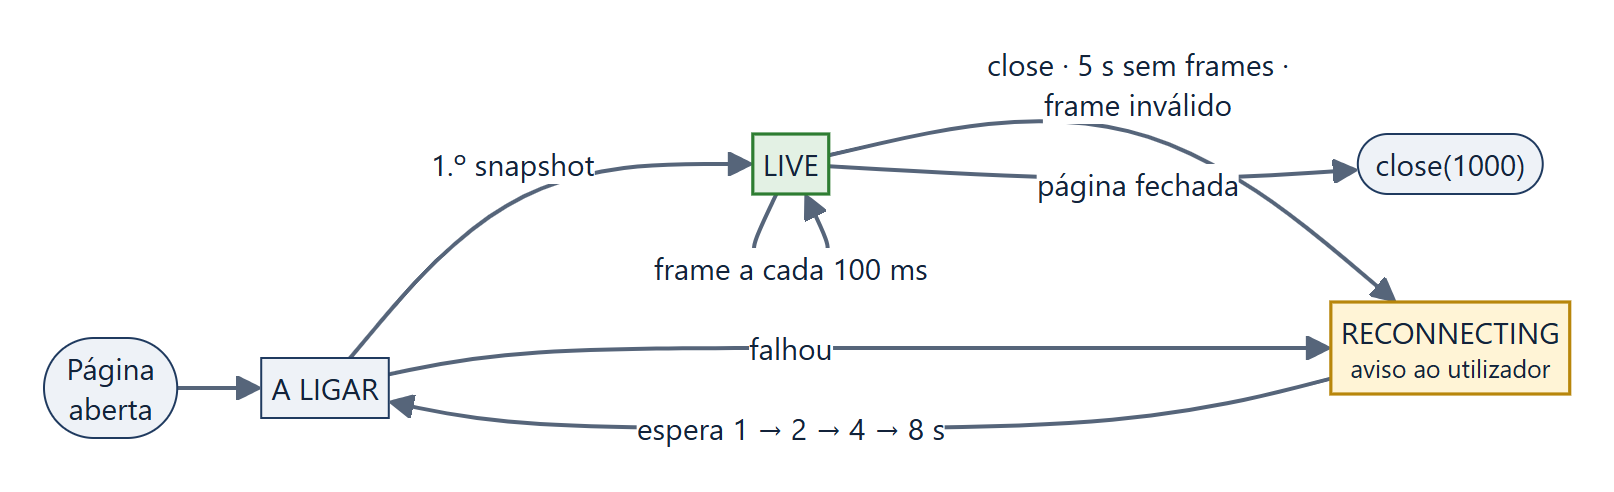
\includegraphics[width=\textwidth]{figuras/websocket_estados.png}
\caption{Estados do canal no \ing{browser}}
\label{fig:ws-estados}
\end{figure}

\paragraph{Desempenho medido.} Com a aplicação a correr e um cliente ligado durante 25 s, chegaram
251 \ing{frames} (10,0 por segundo), com um intervalo médio de 99,8 ms entre \ing{frames}
(desvio-padrão de 11,5 ms) e 33 a 35 KB por \ing{frame}.

\paragraph{Testes do canal.} O publicador tem testes que confirmam que um cliente bloqueado não
atrasa os outros nem a simulação, que um cliente cuja escrita falha é removido e que um cliente
novo recebe logo o último \ing{snapshot}. Um teste de ponta a ponta arranca o servidor real e um
cliente \ing{WebSocket} real e verifica que a travagem de emergência do cenário S8 chega ao cliente
no ciclo em que é inferida, que um cliente religado retoma de imediato e que uma origem estranha é
recusada. No \ing{browser}, os testes Playwright confirmam que a interface se atualiza pelo
\ing{WebSocket} e que recupera sozinha de uma ligação perdida.

Em síntese, o \ing{WebSocket} é o que torna o sistema pericial observável: cada decisão inferida
pelo \ing{Drools} chega à interface no mesmo ciclo, com todas as propostas e a sua explicação, sem
que um \ing{browser} lento ou uma ligação perdida afetem a simulação.

\FloatBarrier
\section{Cenários}\label{sec:cenarios}

Um cenário define o percurso, os atores e as ações temporizadas (por exemplo, mudar o tempo ou pedir uma mudança de via a meio da simulação). Carregar um cenário não dá ao motor acesso ao que nele existe: cada elemento só influencia a decisão depois de detetado. Estão definidos 14 cenários (Tabela 14).

\begin{table}[htbp]
\centering
\small
\caption{Cenários definidos e conhecimento exercitado}\label{tab:cenarios}
\rowcolors{2}{white}{corFundo}
\begin{tabular}{@{}L{0.36\textwidth}L{0.58\textwidth}@{}}
\linhacab \cab{Cenário} & \cab{Conhecimento} \\
S1 Estrada livre & Decisão de base e velocidade de cruzeiro \\
S2 Limite de 90 para 50 km/h & Leitura de sinais e abrandamento a tempo de chegar ao limite \\
S3 Semáforo vermelho & Paragem obrigatória pela distância de travagem; arranque no verde \\
S4 Sinal STOP & Paragem completa de 1,2 s (temporal) e arranque \\
S5 Buraco na via & Desvio para o lado seguro ou redução de velocidade \\
S6 Barreira fechada & Desvio ou paragem antes da barreira \\
S7 Peão a atravessar & Curvas de travagem, paragem e emergência \\
S8 TTC crítico & Janelas temporais (CEP) e travagem de emergência \\
S9 Mudança de via impedida & Encadeamento regressivo e \ing{Why Not} \\
S10 Chuva e baixa aderência & Lógica difusa \\
S11 Cenário sequencial & Várias situações no mesmo percurso \\
S12 Demonstração completa & Percurso de apresentação com ações temporizadas \\
S13 Percurso em matriz & Obstáculos definidos na matriz de vias \\
S14 Ultrapassagem & Ultrapassar um veículo lento e regressar à direita \\
\end{tabular}
\end{table}

Foram escolhidos dois cenários a título de exemplo por serem diferentes entre si e, em conjunto, percorrerem um pouco de todo o sistema: regras normativas e heurísticas, raciocínio temporal, lógica difusa, encadeamento regressivo e os dois canais (velocidade e via). Cada figura mostra a traçagem desde o sensor até à decisão e à explicação.

\subsection{Peão a atravessar (S7)}\label{sec:s7}

O veículo circula a 60 km/h na via central e um peão começa a atravessar 95 m à frente.

\begin{figure}[htbp]
\centering
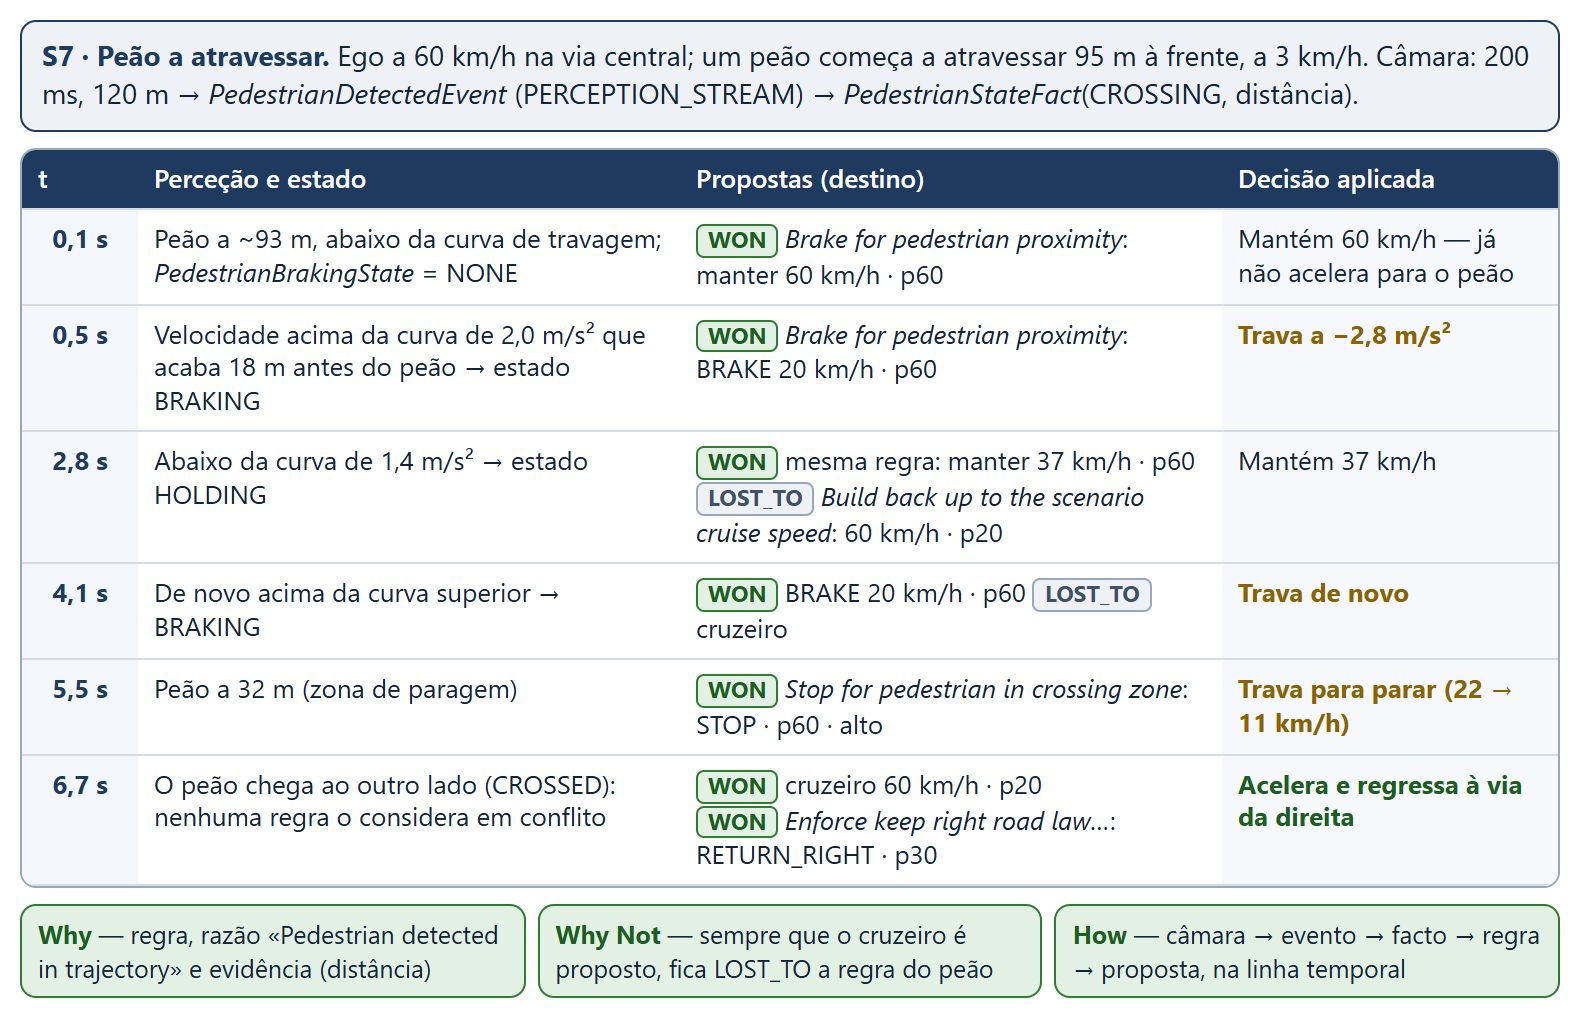
\includegraphics[width=\textwidth]{figuras/tracagem_S7.png}
\caption{Traçagem do cenário S7 --- peão a atravessar}
\label{fig:S7}
\end{figure}

\noindent \textbf{O que demonstra:} conhecimento normativo (ceder passagem) e heurístico (curvas de travagem calculadas, como pediu o perito), estado entre ciclos (PedestrianBrakingState), arbitragem por prioridade e Why com evidência.

\subsection{TTC crítico com chuva (S8)}\label{sec:s8}

O veículo segue a 95 km/h na via central, com outro a 30 km/h 40 m à frente (TTC ≈ 2,2 s); a chuva foi ligada na caixa de ferramentas antes do arranque.

\begin{figure}[htbp]
\centering
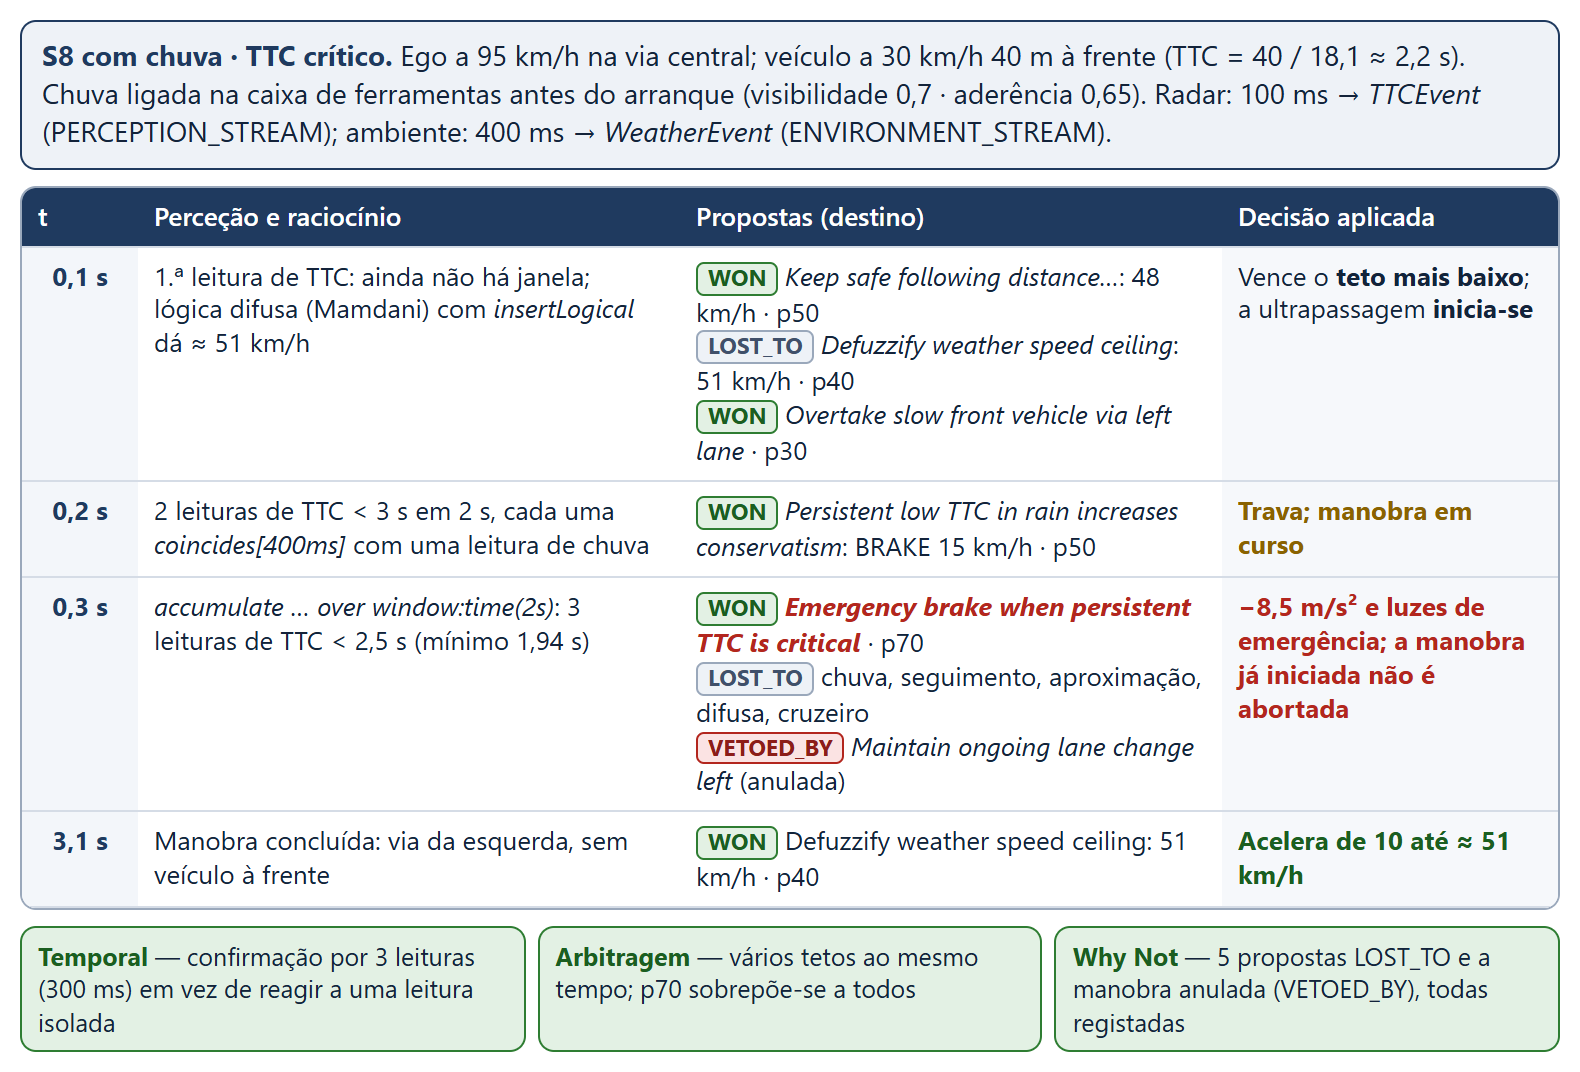
\includegraphics[width=\textwidth]{figuras/tracagem_S8.png}
\caption{Traçagem do cenário S8 com chuva --- TTC crítico, CEP e lógica difusa}
\label{fig:S8}
\end{figure}

\noindent \textbf{O que demonstra:} raciocínio temporal com confirmação adaptada à criticidade, lógica difusa com manutenção da verdade, vários tetos cumpridos em simultâneo e a anulação de uma manobra pelo canal de velocidade.

\FloatBarrier
\section{Testes}\label{sec:testes}

O comportamento foi validado com os cenários anteriores e com testes automáticos com o objetivo de verificar se a decisão respeita as prioridades, que os conflitos têm o vencedor esperado e que situações iguais produzem decisões iguais. Como critérios de aceitação foram usados:

\begin{itemize}
  \item os factos na memória de trabalho que correspondem ao que os sensores detetaram;
  \item a decisão respeita as prioridades e, em conflito, vence a alternativa esperada;
  \item o sistema acompanha a evolução do cenário ao longo do tempo;
  \item cada decisão é explicável pela regra e pela evidência que lhe deram origem;
  \item situações iguais produzem decisões iguais, em execuções repetidas.
\end{itemize}

Validado o comportamento, o capítulo seguinte discute para quem este sistema é útil, o que ainda o
limita e como pode evoluir.
